%% ============================================================
%%  SECCIÓN X — Gráficas
%% ===========================================================

\section{Gráficas}

\begin{figure}[H]
    \centering
    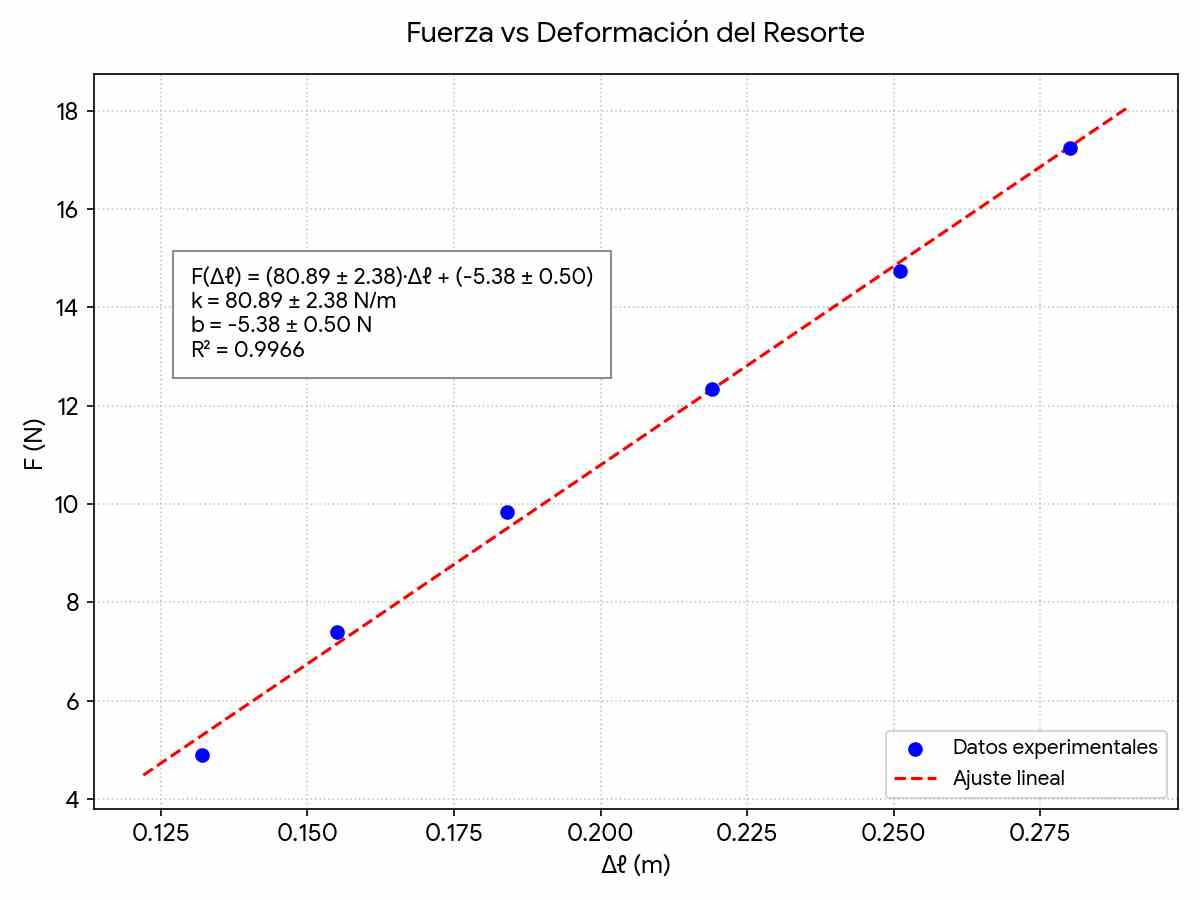
\includegraphics[width=0.85\linewidth]{Figures/Grap1}
    \caption{Fuerza aplicada $F$ en función de la deformación longitudinal
             $\Delta\ell$ del resorte metálico. El ajuste lineal por mínimos
             cuadrados entrega $k = \qty{80{,}89 \pm 2{,}38}{N/m}$,
             con $R^2 = 0{,}9966$.}
    \label{fig:F_resorte}
\end{figure}

\begin{figure}[H]
    \centering
    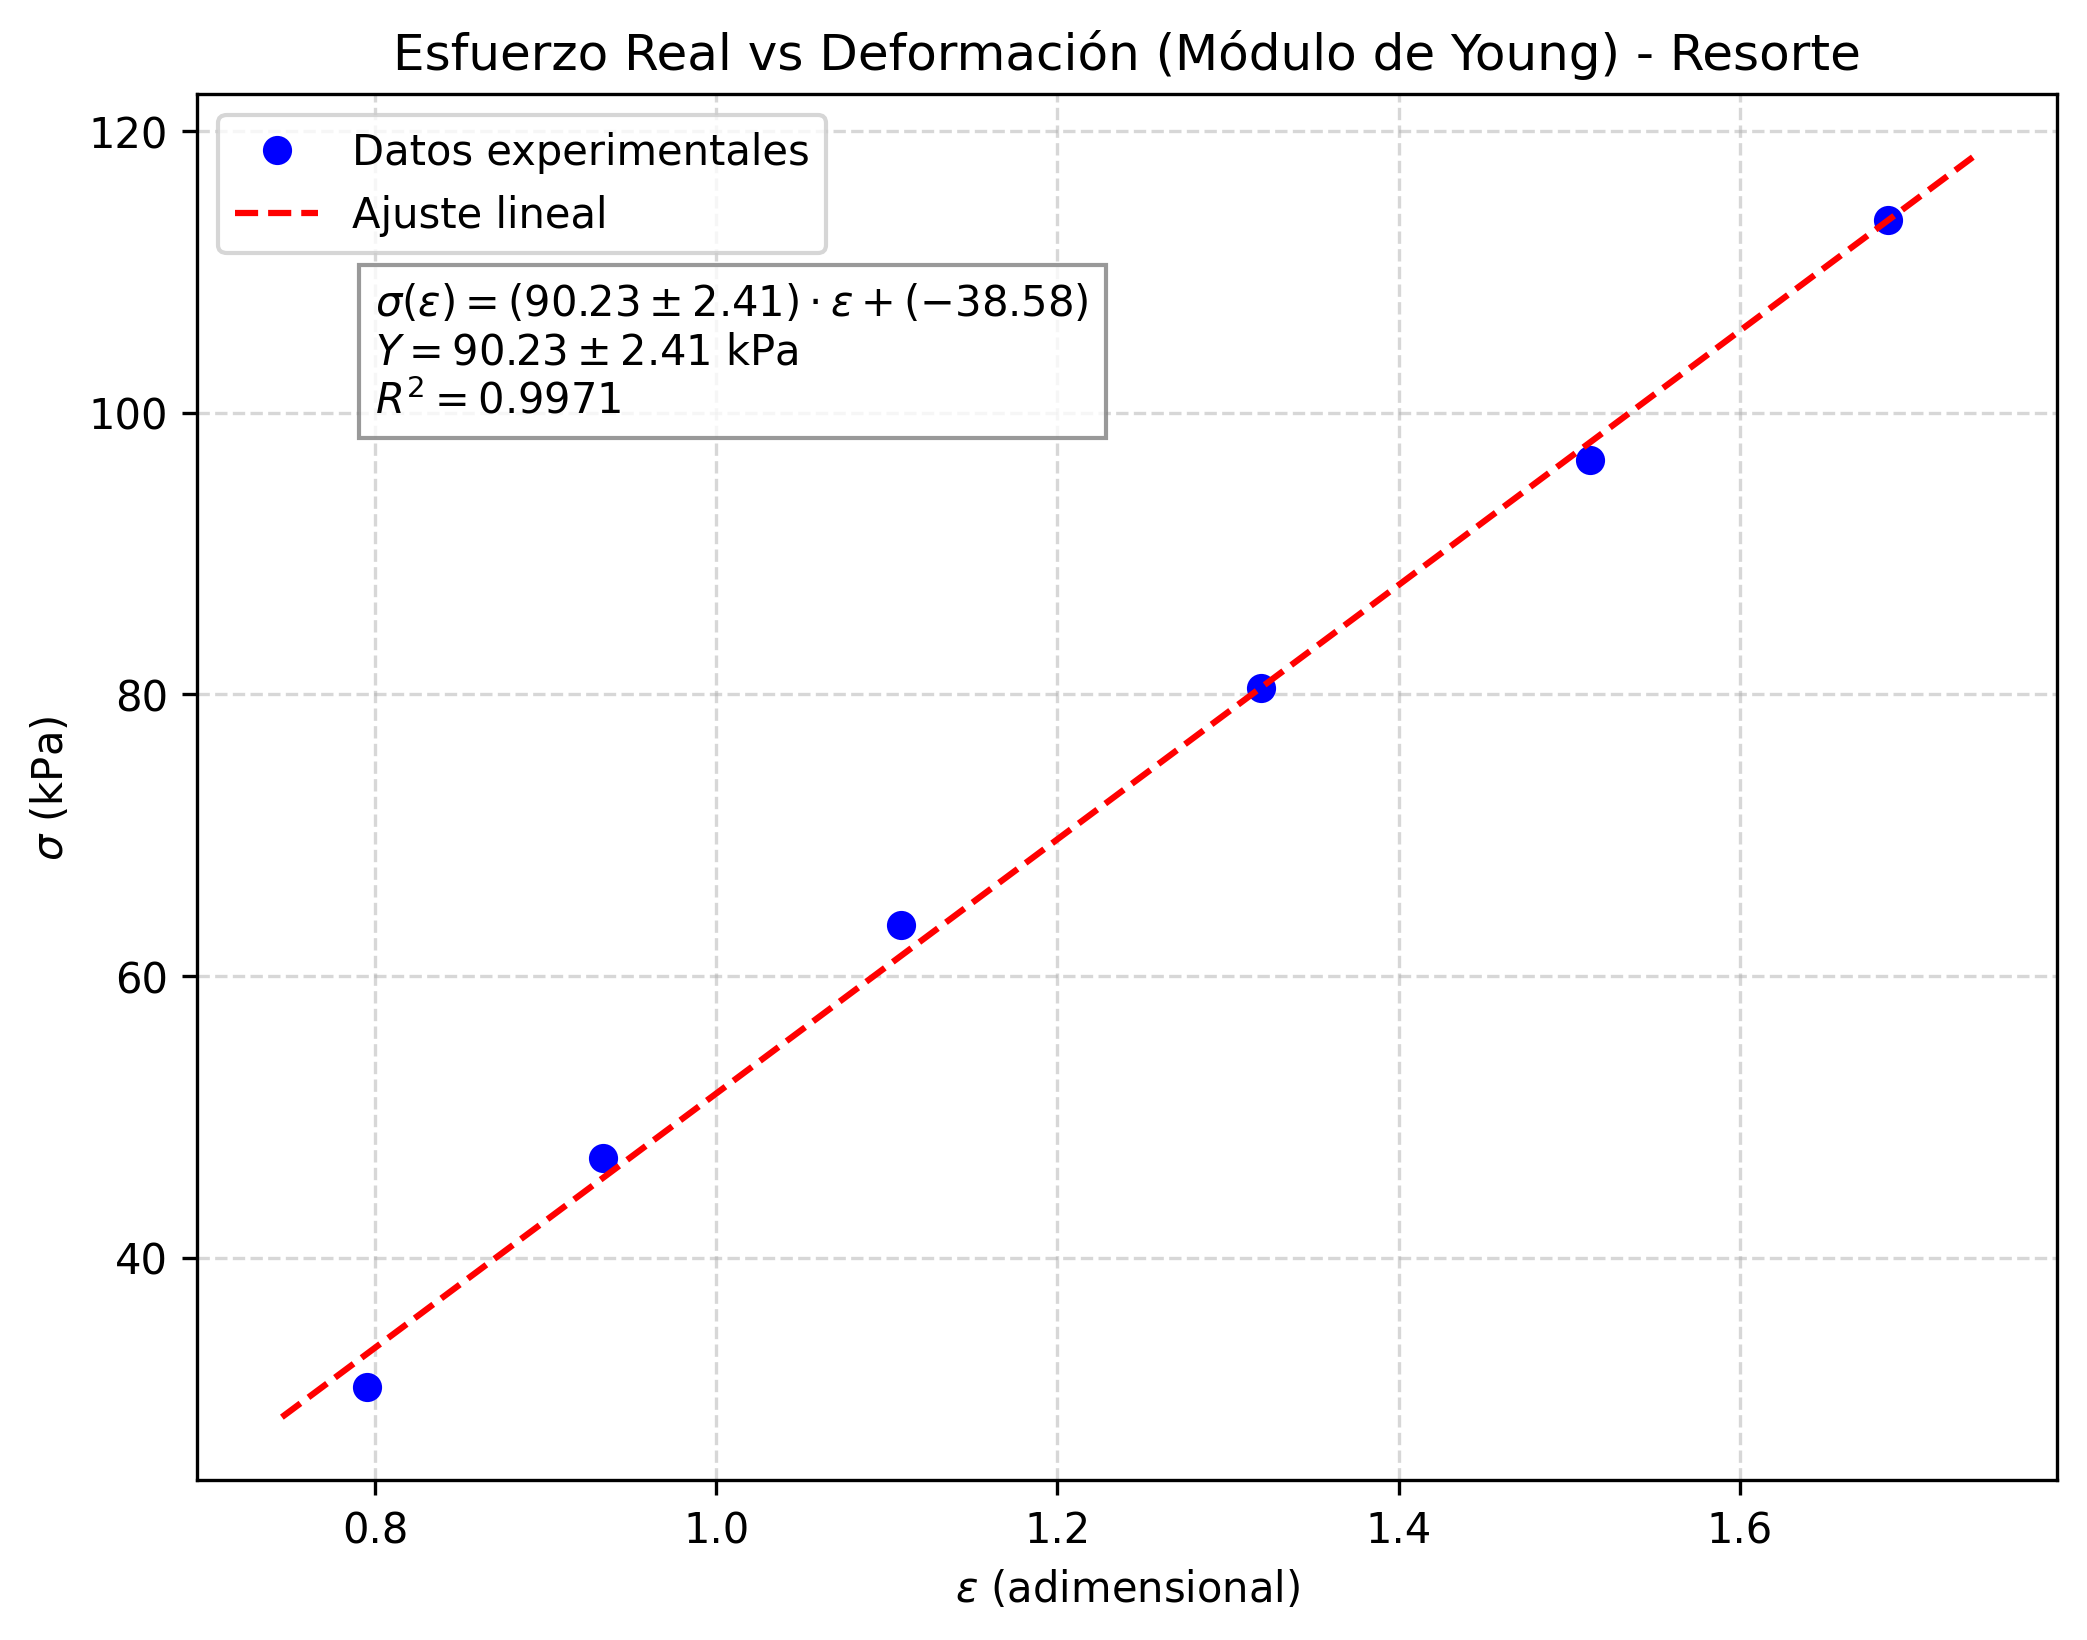
\includegraphics[width=0.85\linewidth]{Figures/Grap2}
    \caption{Diagrama de esfuerzo \textbf{real} versus deformación 
             ($\sigma$ vs.\ $\varepsilon$) del resorte metálico. La pendiente 
             del ajuste lineal corresponde al módulo de Young experimental 
             $Y_r = \qty{90{,}23 \pm 2{,}41}{kPa}$, con $R^2 = 0{,}9971$.}
    \label{fig:sigma_resorte}
\end{figure}

\begin{figure}[H]
    \centering
    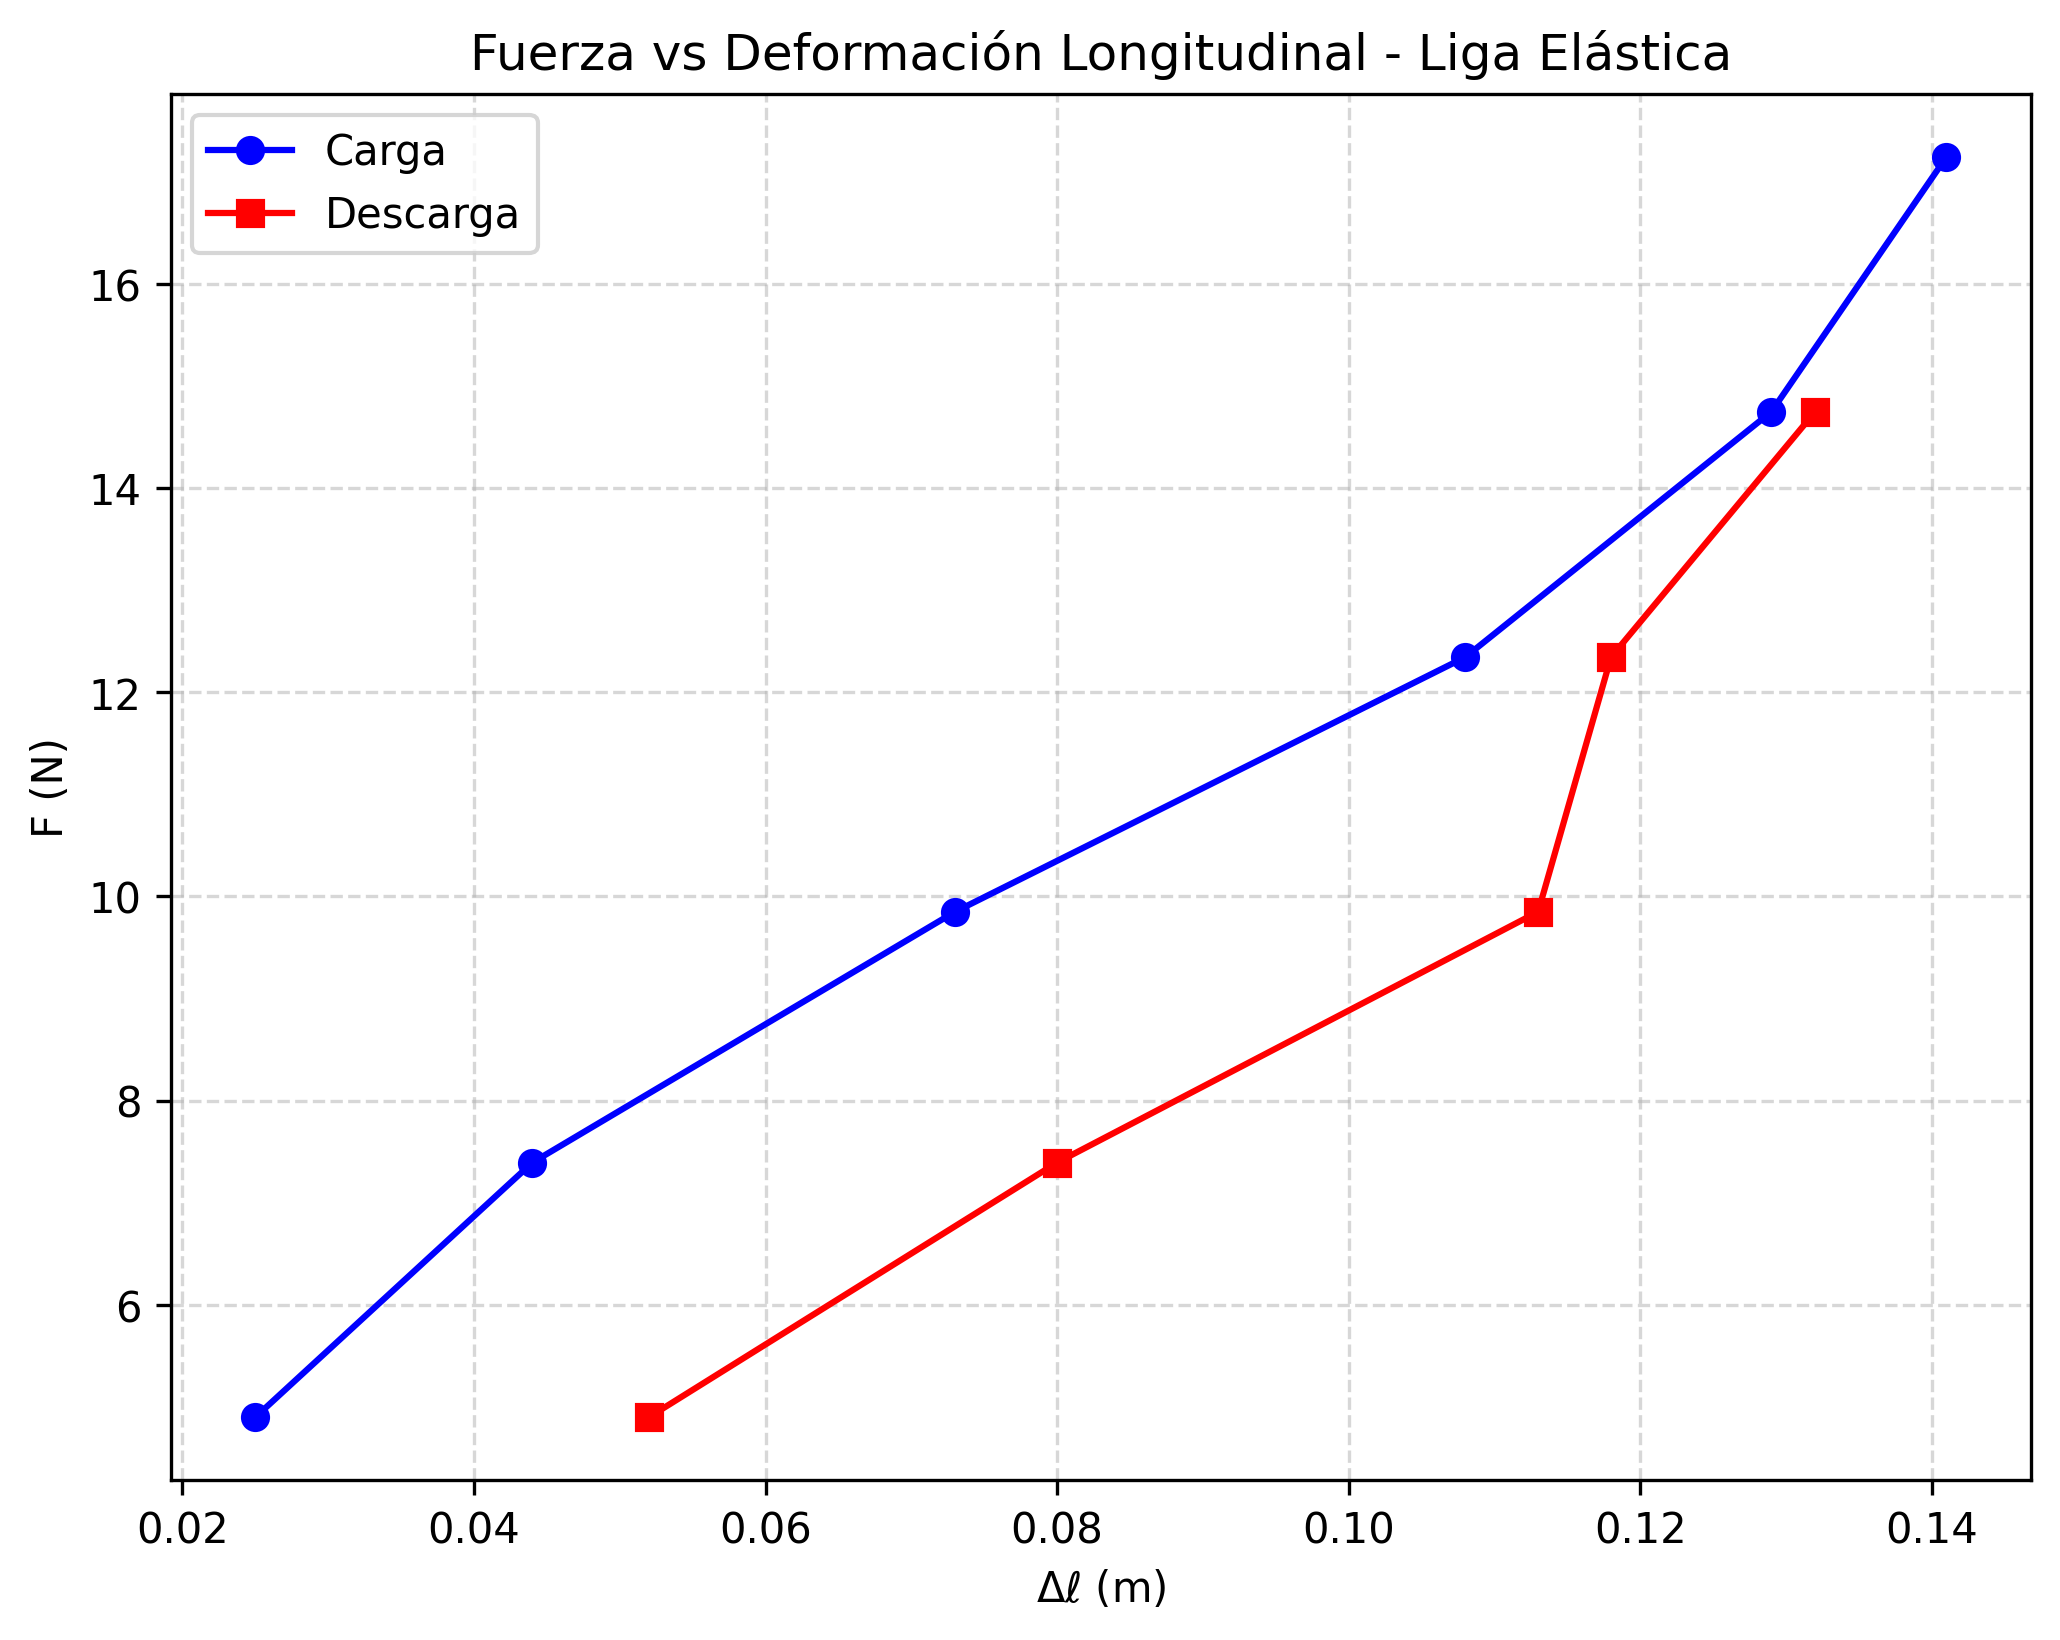
\includegraphics[width=0.85\linewidth]{Figures/Grap3}
    \caption{Fuerza aplicada $F$ en función de la deformación longitudinal
             $\Delta\ell$ de la liga elástica. Se superponen las fases de 
             carga y descarga para evidenciar cualitativamente la existencia 
             de histéresis elástica y deformación remanente.}
    \label{fig:F_liga}
\end{figure}

\begin{figure}[H]
    \centering
    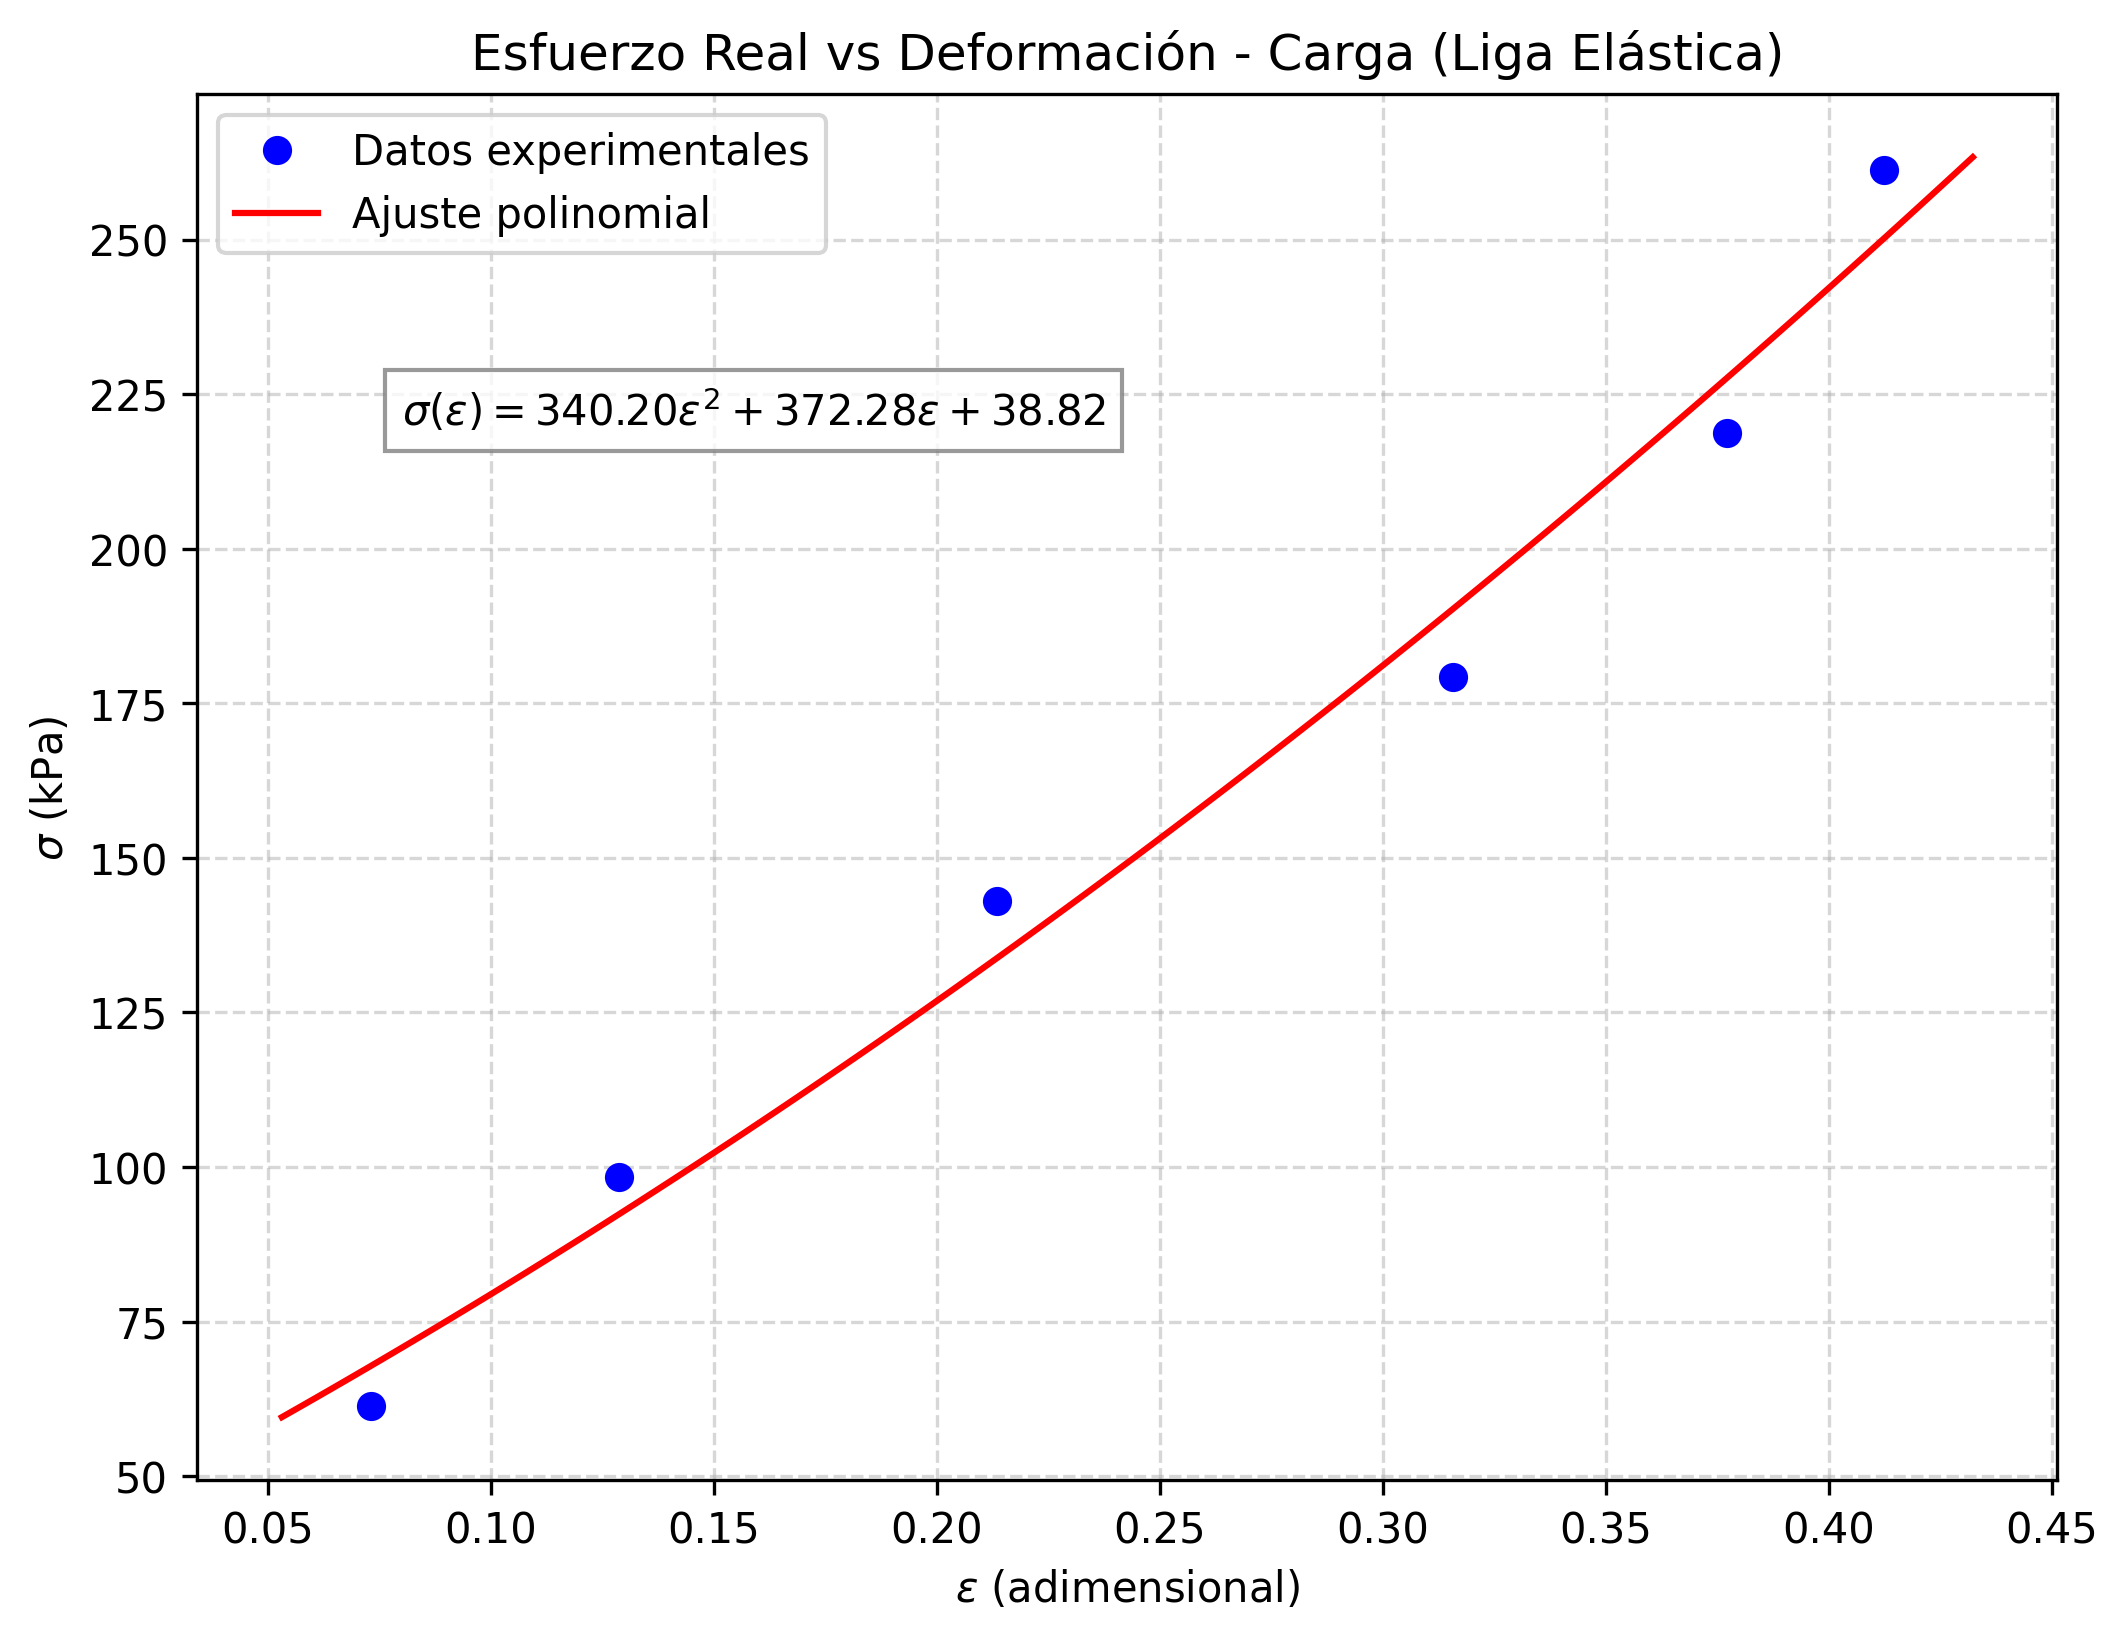
\includegraphics[width=0.85\linewidth]{Figures/Grap4}
    \caption{Diagrama de esfuerzo \textbf{real} versus deformación ($\sigma$ vs.\ $\varepsilon$) de la
             liga elástica durante el proceso de \textbf{carga}. Se presenta un 
             ajuste polinomial de grado~2 ($\sigma = 340{,}20\,\varepsilon^2 + 372{,}28\,\varepsilon + 38{,}82$ kPa), 
             que modela adecuadamente el endurecimiento del material provocado 
             por la contracción transversal.}
    \label{fig:sigma_liga_carga}
\end{figure}

\begin{figure}[H]
    \centering
    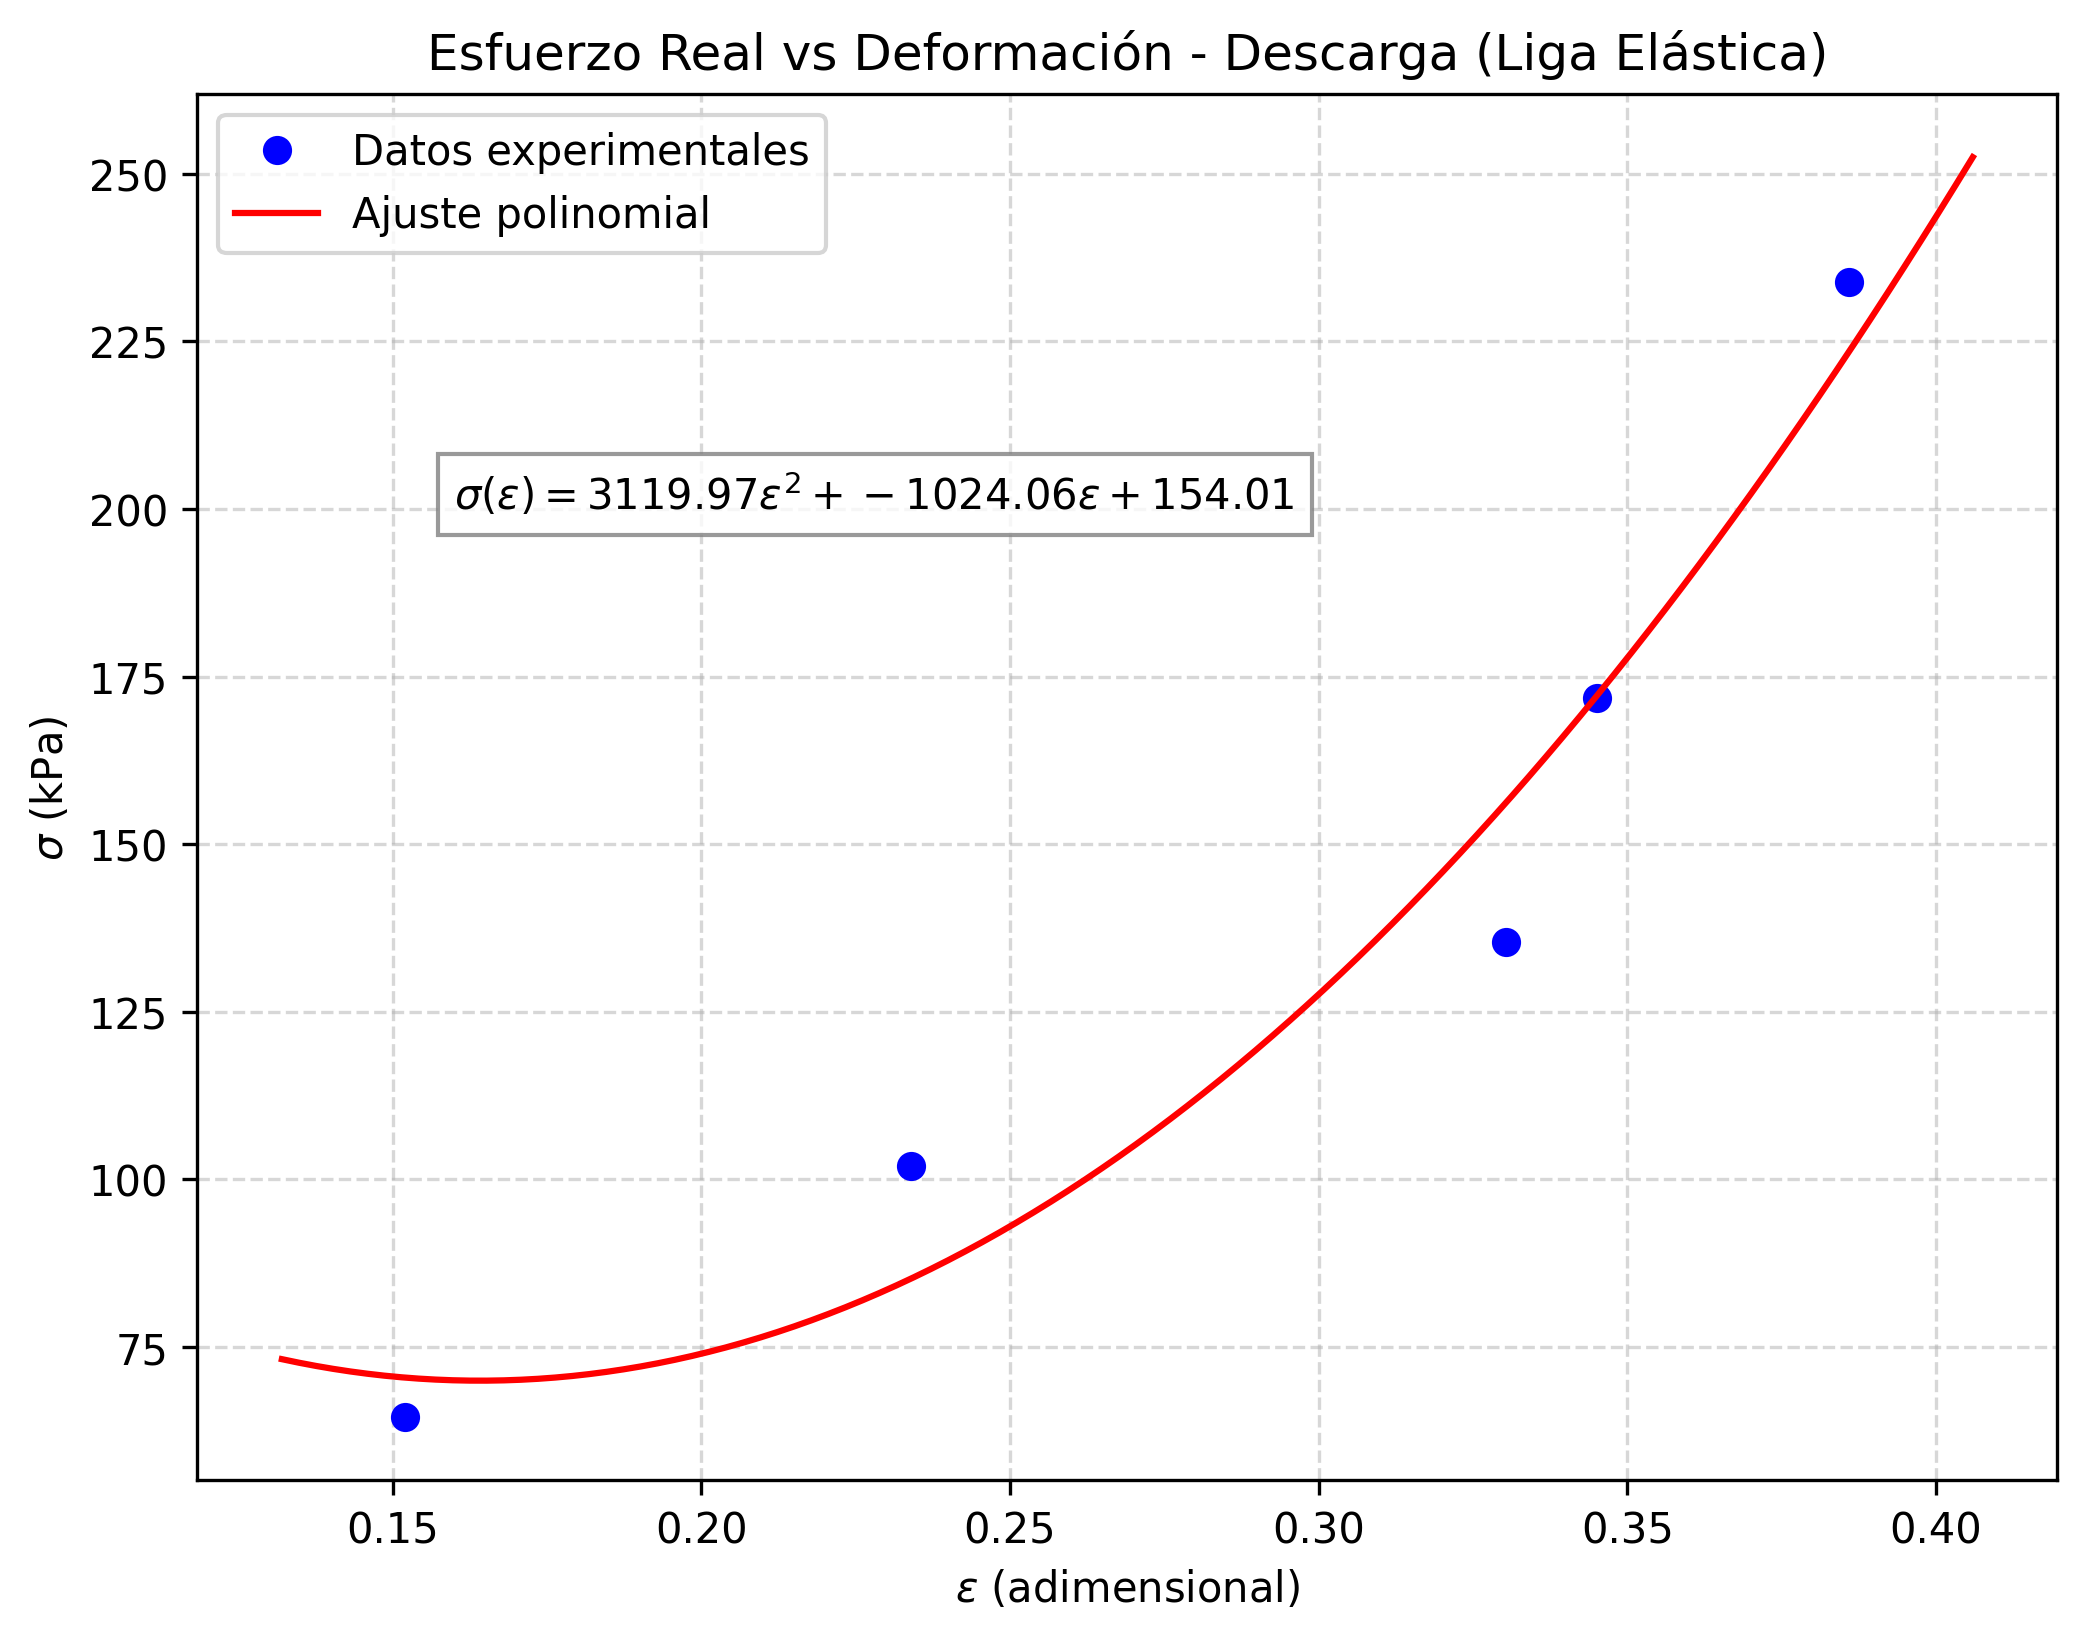
\includegraphics[width=0.85\linewidth]{Figures/Grap5}
    \caption{Diagrama de esfuerzo \textbf{real} versus deformación ($\sigma$ vs.\ $\varepsilon$) de la
             liga elástica durante el proceso de \textbf{descarga}. El ajuste
             polinomial de grado~2 que describe la recuperación es:
             $\sigma = 3119{,}97\,\varepsilon^2 - 1024{,}06\,\varepsilon + 154{,}01$ kPa.}
    \label{fig:sigma_liga_descarga}
\end{figure}

\begin{figure}[H]
    \centering
    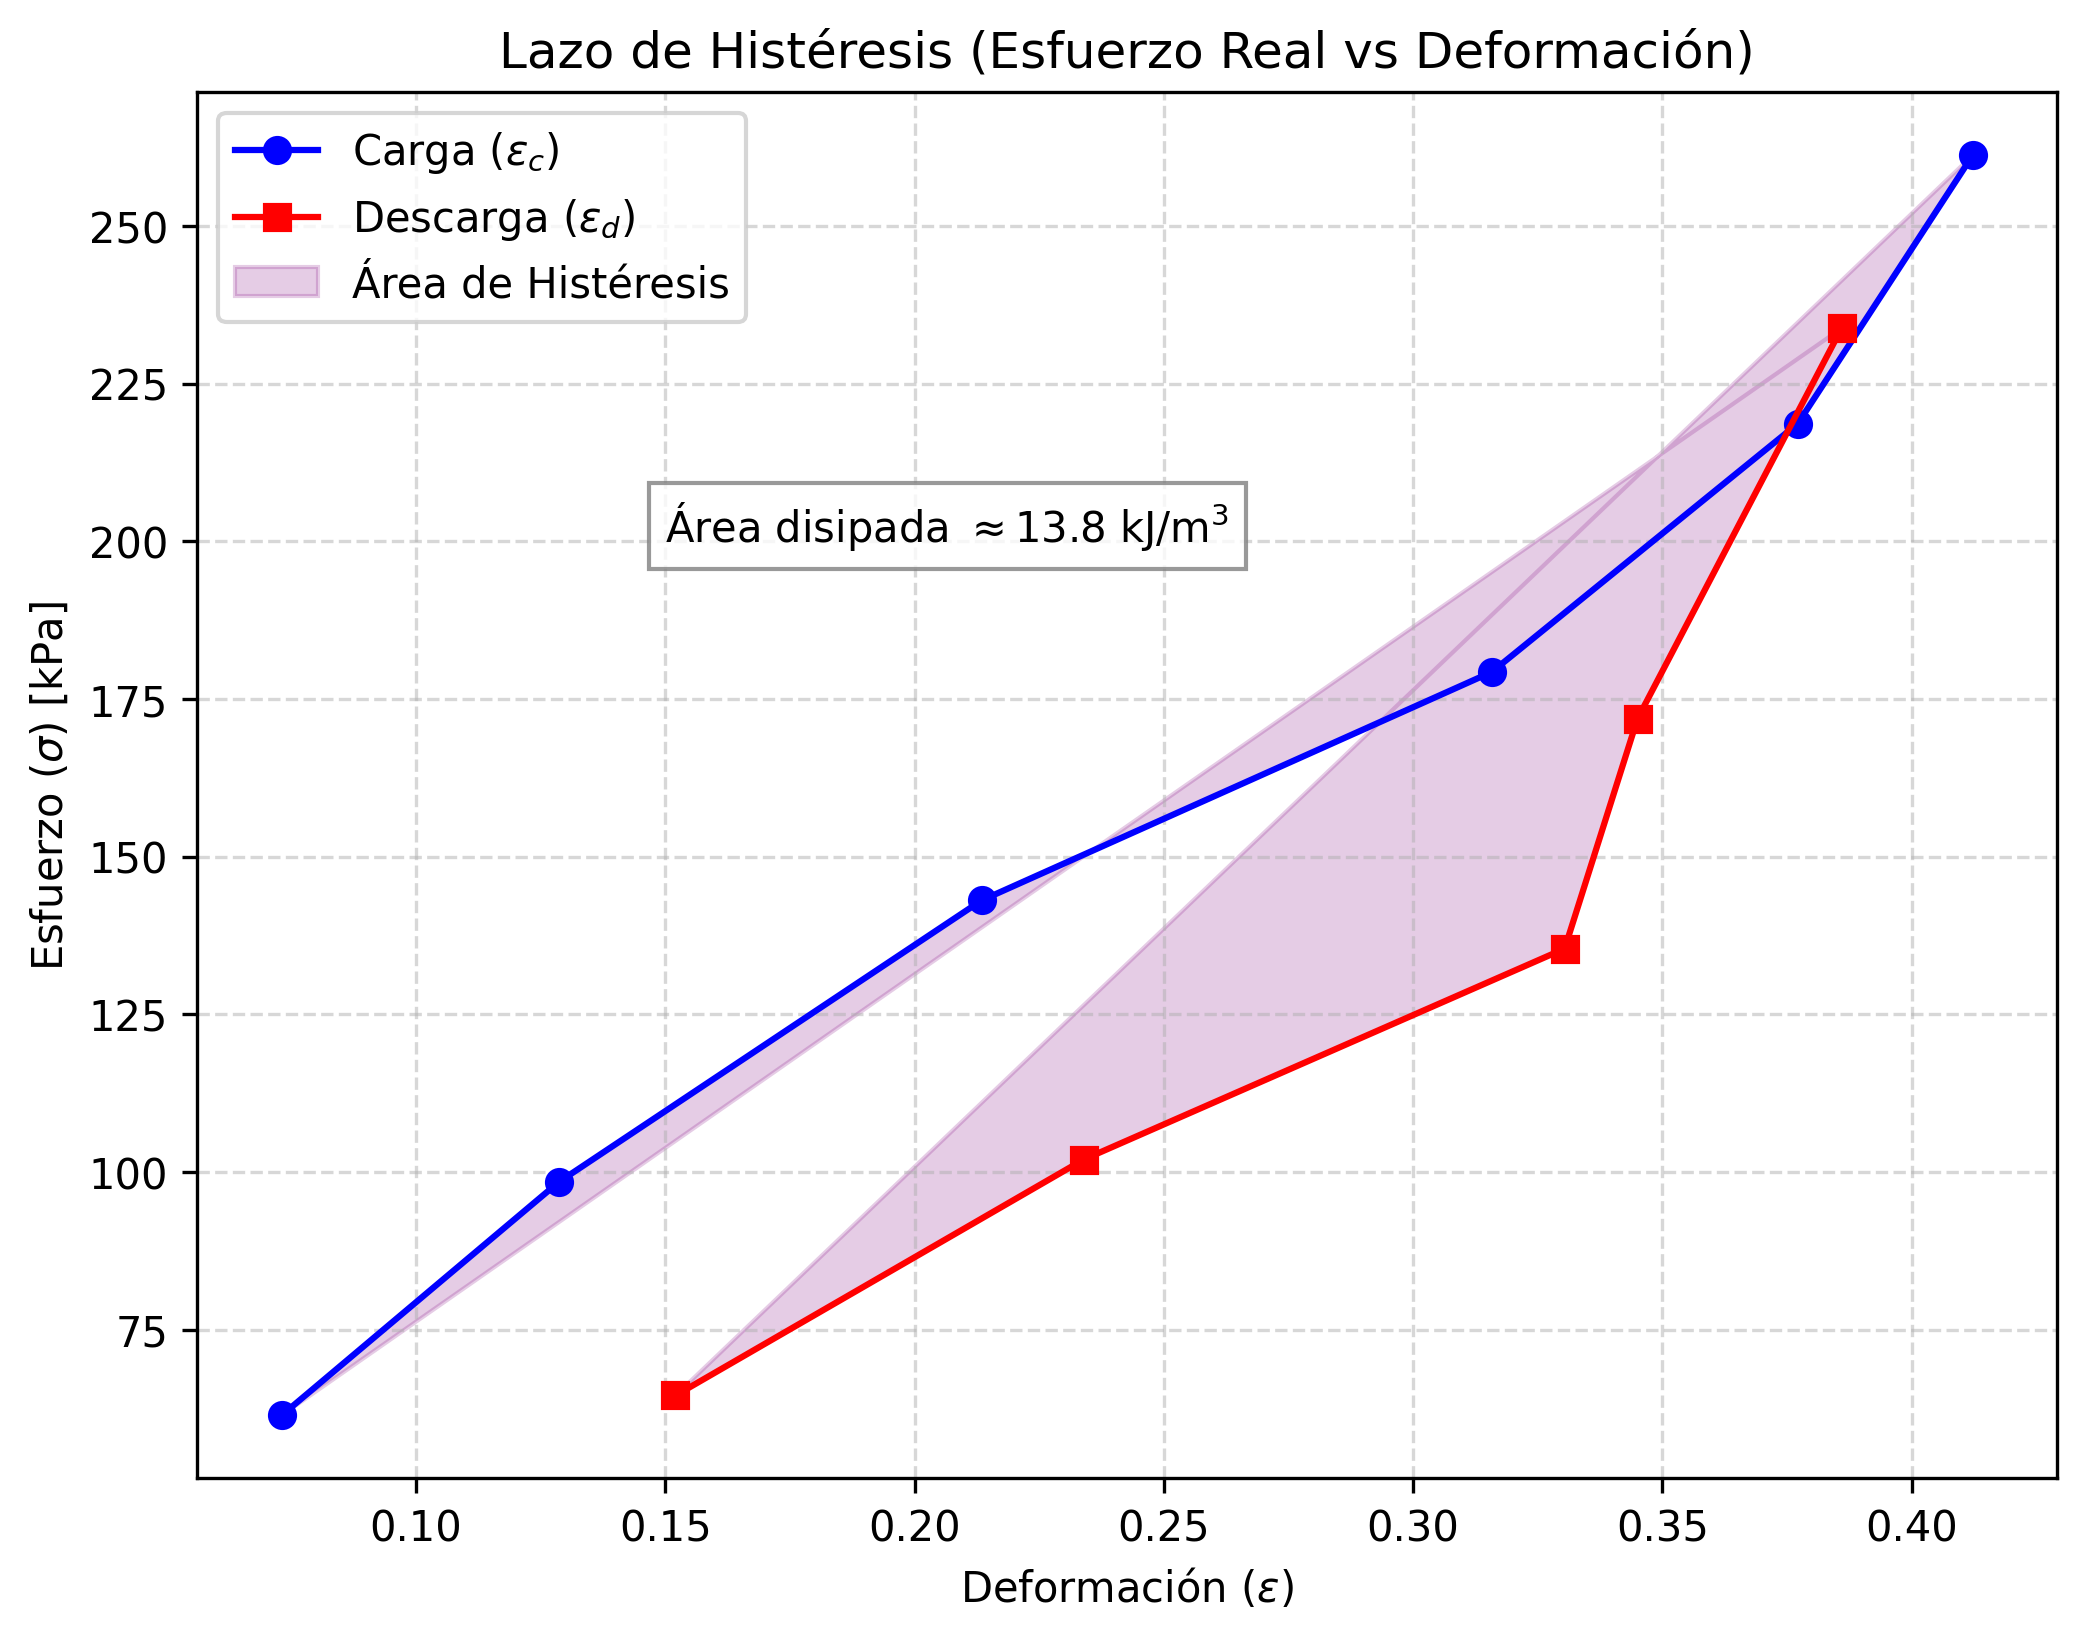
\includegraphics[width=0.85\linewidth]{Figures/Grap6}
    \caption{Lazo de histéresis de la liga elástica en el diagrama de esfuerzo real 
             ($\sigma$--$\varepsilon$). El área sombreada representa
             la energía mecánica disipada internamente por unidad de volumen durante el ciclo
             completo de tracción y recuperación, estimada en
             $A \approx \qty{13{,}8}{kJ/m^3}$.}
    \label{fig:histeresis_lazo}
\end{figure}